% !TEX program = pdflatex
\documentclass[9pt]{extarticle}
\usepackage[letterpaper,margin=0.58in,top=0.64in,bottom=0.58in]{geometry}
\usepackage[T1]{fontenc}
\usepackage{lmodern}
\usepackage{graphicx}
\usepackage{amsmath}
\usepackage{booktabs}
\usepackage{tabularx}
\usepackage{array}
\usepackage{caption}
\usepackage{xcolor}
\usepackage{fancyhdr}
\usepackage{titlesec}
\usepackage{enumitem}
\usepackage{multicol}
\usepackage{hyperref}
\usepackage{microtype}
\usepackage{ragged2e}

\definecolor{navy}{HTML}{193946}
\definecolor{teal}{HTML}{0A7C74}
\definecolor{lightteal}{HTML}{E8F2F1}
\definecolor{amber}{HTML}{D67A35}
\definecolor{lightamber}{HTML}{FFF4E8}
\definecolor{red}{HTML}{B94A48}
\definecolor{lightred}{HTML}{FCEEEE}
\definecolor{slate}{HTML}{526C75}
\definecolor{rulegray}{HTML}{C9D7DA}
\definecolor{lightblue}{HTML}{EEF4F7}

\hypersetup{colorlinks=true,urlcolor=teal,linkcolor=teal}
\pagestyle{fancy}
\fancyhf{}
\lhead{\textcolor{slate}{ECG grouped audit}}
\rhead{\textcolor{slate}{Explanation and improvement script}}
\cfoot{\textcolor{slate}{\thepage\ / 8}}
\renewcommand{\headrulewidth}{0.35pt}
\renewcommand{\footrulewidth}{0pt}
\setlength{\headheight}{12pt}
\setlength{\parindent}{0pt}
\setlength{\parskip}{3pt}
\setlist[itemize]{leftmargin=1.2em,itemsep=1.7pt,topsep=2pt}
\setlist[enumerate]{leftmargin=1.45em,itemsep=2pt,topsep=2pt}
\titleformat{\section}{\large\bfseries\color{navy}}{}{0pt}{}
\titlespacing*{\section}{0pt}{5pt}{3pt}
\newcolumntype{Y}{>{\RaggedRight\arraybackslash}X}
\newcolumntype{L}[1]{>{\RaggedRight\arraybackslash}p{#1}}
\newcolumntype{C}[1]{>{\centering\arraybackslash}p{#1}}
\newcolumntype{R}[1]{>{\raggedleft\arraybackslash}p{#1}}

\newcommand{\pageheading}[2]{%
  {\fontsize{18}{20}\selectfont\bfseries\color{navy} #1}\par
  {\small\color{slate} #2}\par\vspace{3pt}\color{rulegray}\hrule\color{black}\vspace{5pt}
}
\newcommand{\say}[1]{%
  \noindent\fcolorbox{teal}{lightteal}{\parbox{0.965\linewidth}{\textbf{Say aloud}\quad #1}}\par
}
\newcommand{\warningbox}[1]{%
  \noindent\fcolorbox{amber}{lightamber}{\parbox{0.965\linewidth}{\textbf{Important guardrail}\quad #1}}\par
}
\newcommand{\actionbox}[1]{%
  \noindent\fcolorbox{navy}{lightblue}{\parbox{0.965\linewidth}{\textbf{Action implied by the evidence}\quad #1}}\par
}
\newcommand{\metric}[2]{\textbf{#1}: #2}

\begin{document}

% -----------------------------------------------------------------------------
% PAGE 1
% -----------------------------------------------------------------------------
\pageheading{How to explain the ECG audit honestly and clearly}{A 12--15 minute clinician-facing script, with evidence, limitations and a repair plan}

\say{``We tested whether a 52-feature ECG matrix can separate five clinically relevant labels: artifact, seizure, abnormal beat, active noise and strictly unusable signal. The answer is mixed. Artifact and unusable-signal classification look strong inside this dataset. Abnormal-beat classification is useful but inconsistent between patients. Seizure classification is weak and produces many false alarms. Active-noise classification looks strong, but it is supported by only two source patients. These are internal grouped backtest results, not proof of clinical readiness.''}

\section*{The one-sentence conclusion}
\noindent\fcolorbox{red}{lightred}{\parbox{0.965\linewidth}{\large\bfseries The model did not predict everything correctly: the five selected tasks produced 7,162 target-level errors, and the highest scores occur in some of the smallest or least diverse cohorts.}}

\section*{How to use this script}
\begin{tabularx}{\linewidth}{@{}L{1.25in}Y@{}}
\toprule
Marker & Meaning \tabularnewline
\midrule
\textbf{Say aloud} & A ready-to-read explanation written for a clinical audience. \tabularnewline
\textbf{Evidence} & The exact denominator, confusion counts or patient-group distribution supporting the statement. \tabularnewline
\textbf{Guardrail} & A claim that the present data do not justify. \tabularnewline
\textbf{Action} & The next improvement that follows from the observed failure, not from guesswork. \tabularnewline
\bottomrule
\end{tabularx}

\section*{Opening roadmap}
\say{``I will first explain how the data and labels were built, then define the statistics in ordinary language. I will show the overall results, examine whether they hold across independent patient or source groups, and study what happens when abnormal beats and noise occur together. Finally, I will show five weak cases and a stepwise plan for improving both the data and the model.''}

\section*{Five headline findings}
\begin{enumerate}
\item \textbf{Seizure is the urgent weakness:} sensitivity 63.0\%, specificity 71.0\%, and PPV only 19.7\%; 2,960 of 3,688 positive alerts were false.
\item \textbf{Abnormal-beat performance is heterogeneous:} group BA 80.0\%, but six of 40 mixed-class lineages fell below 60\% BA.
\item \textbf{Noise and abnormal morphology interact:} noise sensitivity fell from 76.6\% on normal beats to 60.0\% on abnormal beats.
\item \textbf{Artifact and unusable scores are encouraging, not definitive:} only 17 and 15 lineage groups were available, and eight unusable-signal groups contained only one class.
\item \textbf{The matrix passed strong integrity checks, but shortcut risk remains:} feature missingness alone retained substantial predictive signal, especially for seizure and unusable signal.
\end{enumerate}

\warningbox{Do not summarize this audit as ``97\% accurate.'' The 97.0\% figure is group balanced accuracy for one narrow unusable-signal task. It does not describe seizure, abnormal beats, all artifacts, or end-to-end clinical detection.}

\vfill
{\scriptsize\color{slate}\textbf{Speaker note:} If time is short, present pages 1, 3, 5, 7 and 8. Keep pages 2, 4 and 6 available for questions about methods, patient variability and concrete failures.}

\newpage

% -----------------------------------------------------------------------------
% PAGE 2
% -----------------------------------------------------------------------------
\pageheading{What was actually tested}{The labels, independence unit and statistics determine what the results mean}

\section*{Data and experiment design}
\say{``The complete matrix contains 39,664 unique ECG feature rows from 299 records, 278 subject identifiers and 266 patient/source lineages. Each row has 52 numeric features grouped into four branches: rhythm and heart-rate variability; beat morphology; conduction and repolarization; and signal quality. The matrix also preserves 56 label and provenance fields. We evaluated five targets, five model families and all 15 non-empty feature-branch combinations, giving 375 experiments.''}

\begin{tabularx}{\linewidth}{@{}L{1.25in}Y Y@{}}
\toprule
Target & Class 0 & Class 1 \tabularnewline
\midrule
Artifact & BUT-QDB class 1 or inactive NSTDB interval & BUT-QDB class 2/3 or active NSTDB interval \tabularnewline
Seizure & Outside an expert seizure interval & Inside an expert seizure interval \tabularnewline
Abnormal beat & AAMI N & AAMI S, V, F or Q \tabularnewline
Active noise & Official NSTDB inactive interval & Official NSTDB active-noise interval \tabularnewline
Strict unusable & Pure BUT-QDB class 1 & Pure BUT-QDB class 3; class 2 excluded \tabularnewline
\bottomrule
\end{tabularx}

\warningbox{Unknown labels were excluded for that target, not silently converted to zero. A row can be known for noise but unknown for abnormal beat. This is why target denominators overlap and why their errors must not be interpreted as 7,162 unique patients or episodes.}

\section*{Why the split was grouped}
\say{``Every displayed prediction is out of group: the complete patient or source lineage was excluded from training when its rows were predicted. Imputation and scaling were fitted only on the training fold. This is stricter than a random row split, because neighboring beats from the same patient cannot appear on both sides.''}

\section*{Statistics in plain language}
\begin{tabularx}{\linewidth}{@{}L{1.32in}Y L{2.45in}@{}}
\toprule
Statistic & Plain meaning & Seizure example \tabularnewline
\midrule
Sensitivity & Of all true positives, how many were detected? & $728/(728+428)=63.0\%$ \tabularnewline
Specificity & Of all true negatives, how many were correctly rejected? & $7,230/(7,230+2,960)=71.0\%$ \tabularnewline
PPV / precision & Of all positive alerts, how many were truly positive? & $728/(728+2,960)=19.7\%$ \tabularnewline
Balanced accuracy & Mean of sensitivity and specificity; both classes count equally. & $(63.0\%+71.0\%)/2=67.0\%$ \tabularnewline
Group-macro BA & Calculate performance within each lineage, then average lineages equally. & 67.1\% across three source groups \tabularnewline
Group bootstrap & Resample complete lineages to show group-level uncertainty. & With three groups, apparent precision remains fragile. \tabularnewline
\bottomrule
\end{tabularx}

\section*{What the audit checks proved -- and did not prove}
\begin{itemize}
\item All 4,856 planned raw files (8.15 GB) were byte-read with zero read errors; six isolated rebuilds reproduced all 39,664 row IDs, 52 features and 56 semantic label fields with zero differences.
\item Ten label-semantic checks found zero mismatches. Duplicate feature vectors did not cross lineage groups. All 375 experiment cells retained complete out-of-fold predictions.
\item Training-label permutations returned approximately chance BA. This argues against direct label leakage.
\item These checks establish reproducibility of the matrix and backtest. They do \emph{not} establish transportability to a new hospital, monitor, disease mix or clinical workflow.
\end{itemize}

\vfill
{\scriptsize\color{slate}\textbf{Transition:} ``Now that the denominators and statistics are clear, we can compare the five tasks without confusing a large number of rows with a large number of independent patients.''}

\newpage

% -----------------------------------------------------------------------------
% PAGE 3
% -----------------------------------------------------------------------------
\pageheading{The overall result: five very different levels of evidence}{Diamonds are patient/source-group averages; circles and intervals pool rows while resampling groups}

\begin{center}
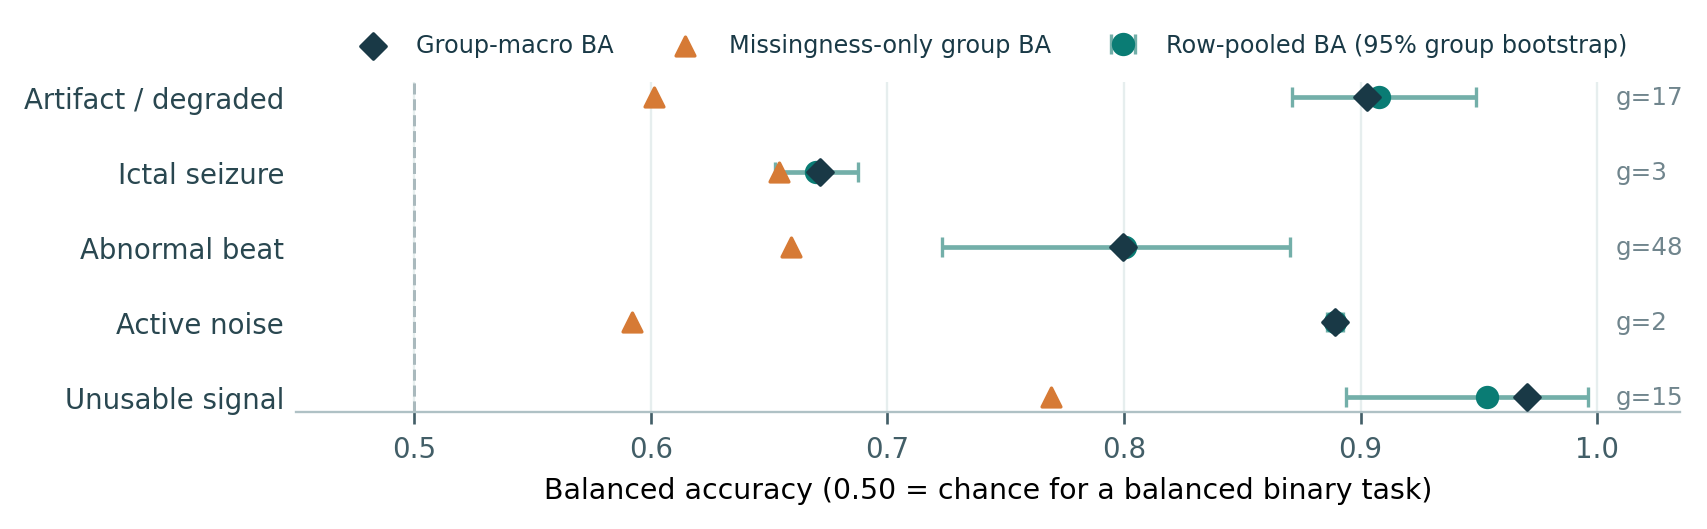
\includegraphics[width=0.97\linewidth]{../clinician_grouped_audit_4page/performance_overview.png}
\end{center}
\vspace{-6pt}

\begin{tabularx}{\linewidth}{@{}L{1.08in}L{1.85in}R{0.46in}R{0.46in}R{0.46in}R{0.52in}R{0.48in}Y@{}}
\toprule
Task & Selected model / branches & Sens. & Spec. & PPV & Group BA & Errors & Interpretation \tabularnewline
\midrule
Artifact & Logistic; B2+B4 & 87.9\% & 93.7\% & 94.5\% & 90.3\% & 1,077 & Strong internal result; 17 groups \tabularnewline
Seizure & Linear SVM; B1 & 63.0\% & 71.0\% & 19.7\% & 67.1\% & 3,388 & Weak; false alarms dominate; 3 groups \tabularnewline
Abnormal beat & Hist. boosting; B1+B2+B3 & 69.9\% & 90.2\% & 64.3\% & 80.0\% & 2,171 & Moderate and heterogeneous; 48 groups \tabularnewline
Active noise & Linear SVM; B2+B4 & 82.2\% & 95.7\% & 97.9\% & 88.9\% & 395 & Strong-looking but only 2 groups \tabularnewline
Strict unusable & Linear SVM; B2 & 92.7\% & 98.0\% & 88.0\% & 97.0\% & 131 & Strong narrow task; 15 groups \tabularnewline
\bottomrule
\end{tabularx}

\section*{Suggested narration}
\say{``The five rows should not be averaged into one score. For artifact, the model detects about 88 of every 100 degraded rows and correctly rejects about 94 of every 100 clean rows. For seizure, it detects only 63 of every 100 ictal rows, rejects only 71 of every 100 non-ictal rows, and only about one in five positive alerts is correct. Abnormal beats sit in the middle: specificity is good, but roughly 30\% of labelled abnormal anchors are missed. Noise and unusable signal appear strong, but their independent-group counts are too small for a clinical generalization claim.''}

\section*{Why the selected branch matters -- but does not settle the science}
\begin{itemize}
\item B1 rhythm/HRV alone won seizure, suggesting the present seizure signal is mainly temporal rather than single-beat morphology.
\item B2 morphology plus B4 quality won artifact and active noise, which is clinically plausible because corruption changes waveform shape and quality measures.
\item B1+B2+B3 won abnormal beat, showing value from rhythm, morphology and conduction together.
\item B2 alone won strict unusable signal. However, the displayed winner was selected from the same 375-cell backtest; it is a comparison winner, not an unbiased final-test estimate.
\end{itemize}

\warningbox{Balanced accuracy is not a clinical operating point. A deployment threshold must be chosen against the actual harm of missed seizures, false alarms, missed abnormal beats and false signal rejection.}

\actionbox{Preserve these models as reproducible baselines. Improve and compare against them using nested group validation, then lock all choices before an untouched external test.}

\vfill
{\scriptsize\color{slate}\textbf{Transition:} ``The aggregate table is only the beginning. We next ask whether the result is consistent from one independent patient or source lineage to another.''}

\newpage

% -----------------------------------------------------------------------------
% PAGE 4
% -----------------------------------------------------------------------------
\pageheading{Patient/source clusters reveal stability and fragility}{A clinically useful model should not depend on a few easy patients or long recordings}

\begin{center}
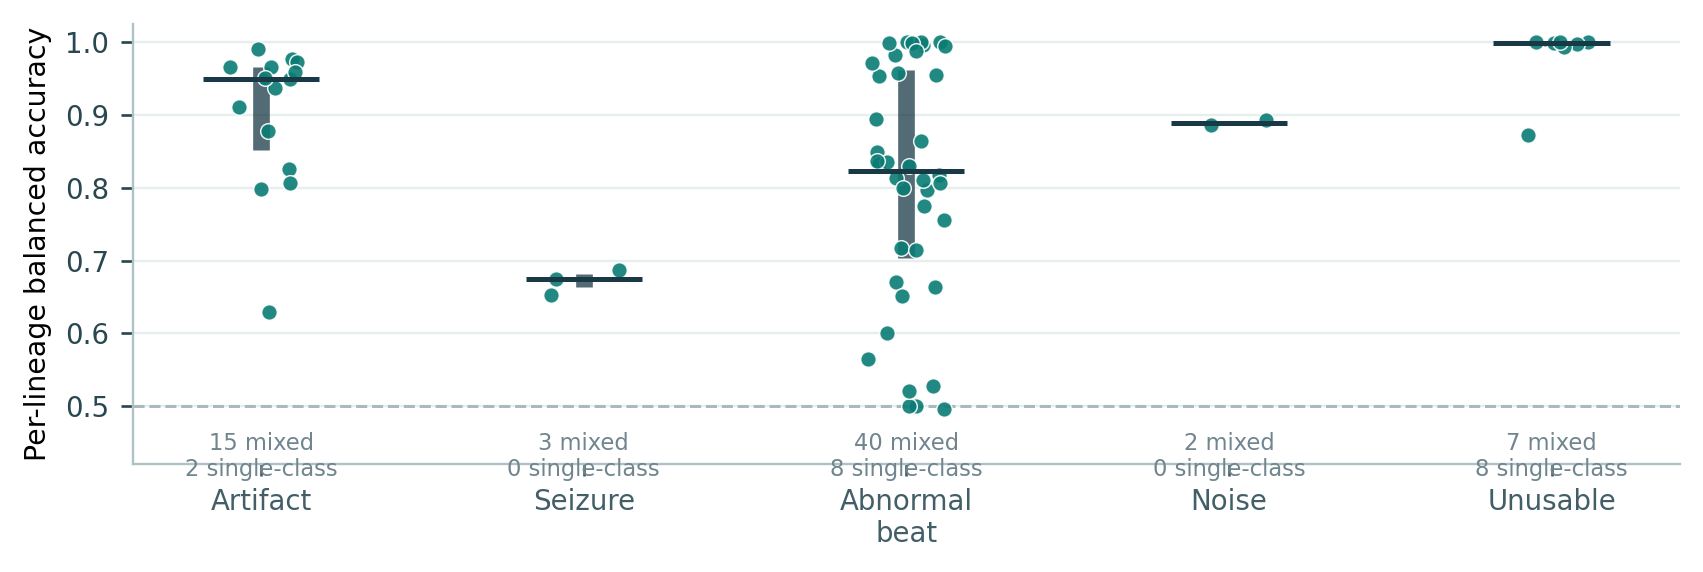
\includegraphics[width=0.96\linewidth]{../clinician_grouped_audit_4page/group_variability.png}
\end{center}
\vspace{-6pt}

\begin{tabularx}{\linewidth}{@{}L{1.05in}C{0.65in}C{0.68in}C{0.78in}C{0.78in}C{0.72in}Y@{}}
\toprule
Task & All groups & Mixed groups & Median BA & IQR & Groups $<60\%$ & What the cluster says \tabularnewline
\midrule
Artifact & 17 & 15 & 95.0\% & 85.2--96.6\% & 0 & Usually stable; worst mixed group 63.0\% \tabularnewline
Seizure & 3 & 3 & 67.4\% & 66.3--68.1\% & 0 & Consistently mediocre; no group reached 80\% \tabularnewline
Abnormal beat & 48 & 40 & 82.3\% & 70.3--96.1\% & 6 & Broad evidence, large patient-to-patient variation \tabularnewline
Active noise & 2 & 2 & 88.9\% & 88.7--89.1\% & 0 & Similar scores do not overcome a two-patient cohort \tabularnewline
Strict unusable & 15 & 7 & 99.9\% & 99.5--100\% & 0 & Seven mixed groups strong; eight cannot test both classes \tabularnewline
\bottomrule
\end{tabularx}

\section*{Suggested narration}
\say{``Each point is an independent patient or source lineage containing both positive and negative examples. The seizure points cluster tightly around 65\% to 69\% balanced accuracy. That tight cluster is not reassuring; it means the current representation is consistently weak across all three source groups. Abnormal-beat performance spans almost chance to perfect, so the 80\% average hides difficult rhythms and records. Artifact is generally stronger but still has a low outlier. Noise has only two points. Strict unusable signal has seven mixed-class points; the other eight groups contain only one class and cannot jointly test sensitivity and specificity.''}

\section*{Three evidence clusters}
\begin{enumerate}
\item \textbf{Broader but heterogeneous: abnormal beats.} Forty-eight lineages provide the best diversity, yet six of 40 mixed groups are below 60\% BA. Improvement must target the difficult subgroup tail, not only the mean.
\item \textbf{Limited but encouraging: artifact and unusable signal.} Their medians are high, but the independent sample counts and single-class groups make the confidence claim narrower than the row counts suggest.
\item \textbf{Critically under-supported: seizure and active noise.} Three and two source groups are not enough to establish transportability, regardless of how many correlated rows they contribute.
\end{enumerate}

\warningbox{A group with only positives can measure sensitivity, and a group with only negatives can measure specificity, but neither can define balanced accuracy alone. Single-class groups must be reported, not discarded or assigned an artificial score.}

\actionbox{Rank future models using group-level performance, confidence intervals and the weak-patient tail. Report the number of independent groups beside every percentage.}

\vfill
{\scriptsize\color{slate}\textbf{Transition:} ``The next question is not only whether each label can be found alone, but whether one condition hides another when labels coexist.''}

\newpage

% -----------------------------------------------------------------------------
% PAGE 5
% -----------------------------------------------------------------------------
\pageheading{Mixed conditions expose clinically important failure modes}{Only combinations with joint ground truth in the same rows can be evaluated honestly}

\begin{center}
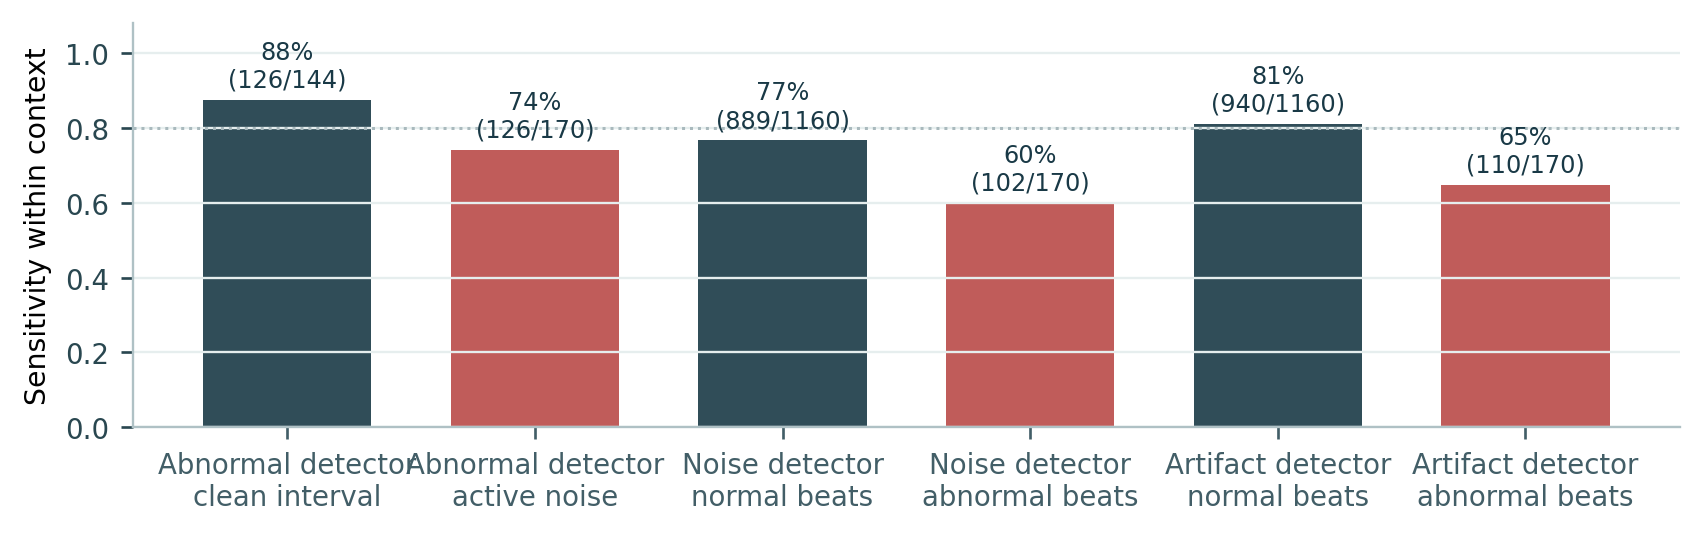
\includegraphics[width=0.96\linewidth]{../clinician_grouped_audit_4page/mixed_context.png}
\end{center}
\vspace{-7pt}

\say{``In the NSTDB rows with both a beat label and a noise schedule, abnormal-beat sensitivity falls from 87.5\% in clean intervals to 74.1\% during active noise. Looking in the other direction, noise sensitivity falls from 76.6\% on normal beats to 60.0\% on abnormal beats. Artifact sensitivity similarly falls from 81.0\% on normal beats to 64.7\% on abnormal beats. This suggests that abnormal morphology and noise can mask one another.''}

\begin{minipage}[t]{0.47\linewidth}
\section*{Jointly labelled NSTDB rows}
\begin{tabular}{@{}lrrr@{}}
\toprule
Context & Normal & Abnormal & Total \\
\midrule
Clean interval & 684 & 144 & 828 \\
Active noise/artifact & 1,160 & 170 & 1,330 \\
\midrule
Total & 1,844 & 314 & 2,158 \\
\bottomrule
\end{tabular}
\end{minipage}\hfill
\begin{minipage}[t]{0.50\linewidth}
\section*{What remains unknown}
Another 689 NSTDB rows keep their official noise/artifact truth but lack an attached abnormal-beat target. They were excluded from the beat cross-tab, not relabelled as normal.

The seizure recordings do not contain synchronized NSTDB noise schedules, AAMI beat labels or BUT-QDB quality consensus. Therefore seizure-plus-noise, seizure-plus-abnormal-beat and seizure-plus-artifact are \textbf{not evaluable} in this matrix.
\end{minipage}

\section*{Why ``not evaluable'' is the correct answer}
\say{``Not evaluable does not mean the combination never occurs and does not mean its performance is zero. It means the required labels were not recorded together. Filling the missing labels with zeros would create a complete-looking but scientifically false matrix.''}

\section*{Quality severity is not one binary concept}
The artifact target combines BUT-QDB class 2 or 3 with active NSTDB noise. Within BUT-QDB, the model correctly rejected 96.1\% of class-1 usable rows, detected 87.8\% of class-2 degraded rows and detected 94.2\% of class-3 unusable rows. The strict unusable task instead compares only class 1 with class 3 and deliberately excludes class 2.

\warningbox{Artifact, active noise and unusable signal overlap conceptually, but they are not interchangeable clinical endpoints. Report the exact label definition and severity class whenever a score is quoted.}

\actionbox{Collect joint annotations prospectively: seizure state, beat class, signal-quality severity, noise type and device/site metadata on the same time windows. Until then, keep unknown targets masked.}

\vfill
{\scriptsize\color{slate}\textbf{Transition:} ``Aggregate and subgroup statistics become easier to understand when we examine individual records where the model clearly failed.''}

\newpage

% -----------------------------------------------------------------------------
% PAGE 6
% -----------------------------------------------------------------------------
\pageheading{Five cases that keep the interpretation honest}{Each example is an out-of-group prediction from a weak record or lineage}

\begin{tabularx}{\linewidth}{@{}L{1.08in}L{1.25in}Y L{2.05in}@{}}
\toprule
Task / record & Confusion counts & Statistical reading & What to say \tabularnewline
\midrule
Seizure\\PN06\_5 & TP 22, FN 49, TN 681, FP 327 & Sensitivity 31.0\%; PPV 6.3\%; BA 49.3\% & ``Only 22 of 71 ictal rows were detected, while 327 non-ictal rows generated alerts. This record is effectively near chance.'' \tabularnewline
Artifact\\NSTDB 118e24 & TP 41, FN 116, TN 72, FP 4 & Sensitivity 26.1\%; specificity 94.7\%; BA 60.4\% & ``The model rarely called artifact falsely, but it missed almost three quarters of actual artifact rows. A negative result is not reassuring here.'' \tabularnewline
Active noise\\NSTDB 118e24 & TP 66, FN 91, TN 65, FP 11 & Sensitivity 42.0\%; specificity 85.5\%; BA 63.8\% & ``The overall 88.9\% group BA hides a record in which most noisy rows were missed.'' \tabularnewline
Abnormal beat\\MIT-BIH 207 & TP 36, FN 67; no negatives in selected window & Sensitivity 35.0\%; specificity undefined & ``Two thirds of abnormal anchors were called normal. With no negative rows here, specificity cannot rescue the result.'' \tabularnewline
Strict unusable\\BUT 111001 & TP 137, FN 47, TN 105, FP 0 & Sensitivity 74.5\%; specificity 100\%; BA 87.2\% & ``There were no false unusable alarms, but one quarter of truly unusable rows received false reassurance.'' \tabularnewline
\bottomrule
\end{tabularx}

\section*{How to connect the cases to the aggregate result}
\say{``These cases are not cherry-picked to discredit the model. They are stress tests showing how an aggregate percentage can fail a particular patient or record. Clinically, false reassurance is often more important than a strong average. The correct response is to explain why these records are difficult, add representative data, and require the next model to improve the weak-group tail.''}

\section*{What each case tells us to fix}
\begin{enumerate}
\item \textbf{PN06\_5 seizure:} optimize for episode-level alerts and false alarms per hour, not isolated row accuracy; add more independent seizure patients and difficult non-ictal rhythms.
\item \textbf{118e24 artifact/noise:} examine noise subtype, amplitude and transition position; train on more devices and source patients; use calibrated uncertainty rather than a hard reassuring negative.
\item \textbf{MIT-BIH 207 abnormal beats:} stratify errors by AAMI class and rhythm; test whether morphology, conduction or detector alignment failed; include missed expert beats in end-to-end evaluation.
\item \textbf{BUT 111001 unusable signal:} target false negatives explicitly and model the ordinal usable/degraded/unusable scale instead of relying only on a binary extreme comparison.
\end{enumerate}

\warningbox{These rows are anchored to detected beats. If the upstream detector misses an expert beat entirely, no classifier row is created. Therefore abnormal-beat sensitivity here is not end-to-end beat-detection sensitivity.}

\section*{A useful answer when asked, ``Which number should I trust?''}
\say{``Trust the full pattern: confusion counts, patient-group distribution, mixed-condition behavior and the weak cases. No single percentage contains all four. The result is credible as an internal audit because the reconstruction and grouped backtest are reproducible, but its clinical scope remains limited.''}

\vfill
{\scriptsize\color{slate}\textbf{Transition:} ``The repair plan should follow these observed errors in priority order, beginning with the data and validation design rather than immediately adding a more complex classifier.''}

\newpage

% -----------------------------------------------------------------------------
% PAGE 7
% -----------------------------------------------------------------------------
\pageheading{How to improve the system based on the statistics}{Every proposed change is tied to an observed weakness and a testable outcome}

\begin{tabularx}{\linewidth}{@{}L{0.72in}L{1.52in}Y Y@{}}
\toprule
Priority & Statistical trigger & Fix & Evidence required next \tabularnewline
\midrule
1 & Seizure: 3 groups, 63.0\% sensitivity, 19.7\% PPV, 2,960 FP & Add independent seizure patients and difficult non-ictal controls; create episode-level labels; calibrate thresholds and temporal alarm persistence inside training folds. & Patient-group CI, episode sensitivity, false alarms/hour, alert duration and untouched external performance. \tabularnewline
1 & Missingness-only group BA: 65.4\% seizure; 76.9\% unusable & Standardize the feature panel; audit why values are absent; compare with and without missingness indicators; test leave-one-dataset/site-out splits. & Gain must remain after harmonized missingness and source-held-out testing. \tabularnewline
2 & Mixed-context drops: noise 76.6\% to 60.0\%; artifact 81.0\% to 64.7\% on abnormal beats & Collect and upweight real jointly labelled abnormal-plus-noise cases; add noise type/severity; test quality-aware or multi-task models with masked unknown labels. & Sensitivity by joint class with adequate independent groups; no deterioration of clean abnormal-beat specificity. \tabularnewline
2 & Abnormal beats: 6/40 mixed groups below 60\% BA; MIT 207 sensitivity 35.0\% & Review errors by AAMI subtype and rhythm; model N/S/V/F/Q separately before optional binary collapse; improve beat anchoring and evaluate missed expert beats. & End-to-end sensitivity per AAMI class, weak-group tail and per-patient confusion matrices. \tabularnewline
3 & Noise: only 2 groups; artifact 17; strict unusable 15 with 8 single-class groups & Add patients, hospitals, devices and naturally occurring motion/electrode artifacts; retain ordinal quality consensus and annotator disagreement. & External group count, subgroup CIs, calibration and device/site held-out results. \tabularnewline
\bottomrule
\end{tabularx}

\section*{Recommended cascade behavior}
\noindent\fcolorbox{navy}{lightblue}{\parbox{0.965\linewidth}{\centering
\textbf{Raw ECG} $\longrightarrow$ \textbf{quality severity + uncertainty} $\longrightarrow$ \textbf{R-peak/beat detection} $\longrightarrow$ \textbf{beat and seizure models} $\longrightarrow$ \textbf{calibrated output: positive / negative / abstain} $\longrightarrow$ \textbf{clinician review}
}}

\say{``The strongest immediate design improvement is not simply a deeper model. The cascade should first estimate quality severity and uncertainty. When the signal is unreliable or unlike training data, it should abstain or request review rather than issue a confident negative. Beat and seizure outputs should then be calibrated for their specific clinical use.''}

\section*{Model-development experiments worth running}
\begin{itemize}
\item Keep the five audited families as baselines. Add temporal models for seizure episodes only after expanding patient-level data; compare them under the same grouped protocol.
\item Use nested grouped cross-validation: inner folds select features, model and threshold; outer folds estimate performance. The present winner-selection optimism is then reduced.
\item Test leave-one-dataset, device or site out. If performance collapses, the model learned acquisition context rather than physiology.
\item Calibrate probabilities on training groups only. Choose operating points using explicit clinical costs and report sensitivity-specificity tradeoffs rather than one default threshold.
\item Add an out-of-distribution or disagreement flag. A safe ``uncertain'' output is preferable to a confident false reassurance on records like 118e24 or BUT 111001.
\end{itemize}

\warningbox{Synthetic augmentation and class weighting may help optimization, but they cannot replace new independent patients or missing joint ground truth. Do not generate labels for combinations that were never annotated.}

\actionbox{Fix the highest-risk evidence gaps first: seizure cohort and false alarms, jointly labelled noisy abnormal beats, and end-to-end beat accounting. Tune model complexity only inside that stronger evaluation design.}

\vfill
{\scriptsize\color{slate}\textbf{Transition:} ``The final step is to define what evidence would count as improvement before seeing the next results.''}

\newpage

% -----------------------------------------------------------------------------
% PAGE 8
% -----------------------------------------------------------------------------
\pageheading{A defensible next-study plan and closing script}{Predefine the test, preserve failures and require evidence at patient level}

\section*{Four phases}
\begin{tabularx}{\linewidth}{@{}L{0.72in}L{1.35in}Y L{2.18in}@{}}
\toprule
Phase & Goal & Required work & Exit evidence \tabularnewline
\midrule
0 & Freeze baseline & Version the current matrix, group map, folds, prediction ledger and five selected baselines. Keep PN06\_5, 118e24, MIT 207 and BUT 111001 as regression cases. & Exact rebuild and current metrics reproduce from a clean environment. \tabularnewline
1 & Repair data & Expand independent groups; annotate seizure, beat type, quality and noise jointly; document unknowns; include detector misses and real clinical negatives. & Label coverage table, adjudication agreement, group counts and no fabricated negatives. \tabularnewline
2 & Develop safely & Nested group selection, missingness/source ablations, episode-level seizure logic, multiclass beats, quality-aware abstention and calibration. & Locked candidate improves group distribution and intended operating metrics, not only row accuracy. \tabularnewline
3 & Test once & Apply the frozen pipeline to an untouched external cohort representing the intended site, device and patient mix. & Patient-level CIs, subgroup results, calibration, errors per hour and complete failure review. \tabularnewline
\bottomrule
\end{tabularx}

\section*{The scorecard to pre-register}
\begin{multicols}{2}
\begin{itemize}
\item Sensitivity, specificity, PPV and NPV with exact denominators.
\item Patient/source group-macro metrics and group bootstrap intervals.
\item Median, interquartile range, worst-group and lower-tail performance.
\item Seizure episode sensitivity, false alarms per hour and detection delay.
\item End-to-end AAMI class sensitivity, including missed detector beats.
\item Performance by quality severity, noise type, beat class, device and site.
\item Probability calibration and abstention/coverage tradeoff.
\item Missing-label coverage and missingness/source-control results.
\end{itemize}
\end{multicols}

\section*{Questions you are likely to receive}
\begin{tabularx}{\linewidth}{@{}L{2.0in}Y@{}}
\toprule
Question & Concise answer \tabularnewline
\midrule
``Why is 97\% not enough?'' & It applies only to strict class-1 versus class-3 unusable signal, not to seizure or all artifacts, and only seven groups contain both classes. \tabularnewline
``Did grouped validation eliminate leakage?'' & It strongly reduces patient overlap and the permutation control is reassuring, but missingness still carries label information and there is no external cohort. \tabularnewline
``Which task is closest to useful?'' & Artifact and strict unusable signal are the strongest internal engineering candidates. Neither is approved for autonomous rejection or diagnosis. \tabularnewline
``What should be fixed first?'' & More independent and jointly labelled seizure/noise/beat data, false-alarm analysis, missingness harmonization and end-to-end beat accounting. \tabularnewline
``Can we report seizure with artifact or abnormal beats?'' & Not from this matrix; those labels were not jointly recorded in the seizure rows. The valid result is ``not evaluable.'' \tabularnewline
\bottomrule
\end{tabularx}

\section*{Closing statement}
\say{``This audit gives us a trustworthy map of what the current matrix can and cannot support. The matrix reconstruction and grouped prediction ledger are reproducible. Artifact and unusable-signal features are promising; abnormal-beat performance is useful for some patients but uneven; seizure is not ready; and noise evidence is too narrow. The next advance should come from broader joint labels, end-to-end evaluation, shortcut controls, calibrated uncertainty and a locked external test. Our goal is not a larger headline number. It is fewer missed clinical events, fewer unnecessary alarms and performance that holds for new patients.''}

\warningbox{Final claim to avoid: ``The model is clinically validated.'' Correct claim: ``The system has passed a reproducible internal grouped audit and has a defined path to external validation.''}

\vfill
{\scriptsize\color{slate}\textbf{Reporting basis:} audit version 2.0.0; 39,664-row matrix SHA-256 \texttt{2e7751f2894343fa367c790f41af2e0f...}; 375 complete out-of-group experiments. Improvement targets must be finalized with clinicians according to intended use and harm, before the next locked evaluation.}

\end{document}
